\documentclass{standalone}

\usepackage{tikz}
\usetikzlibrary{backgrounds}
\usetikzlibrary{decorations.pathreplacing}

\begin{document}
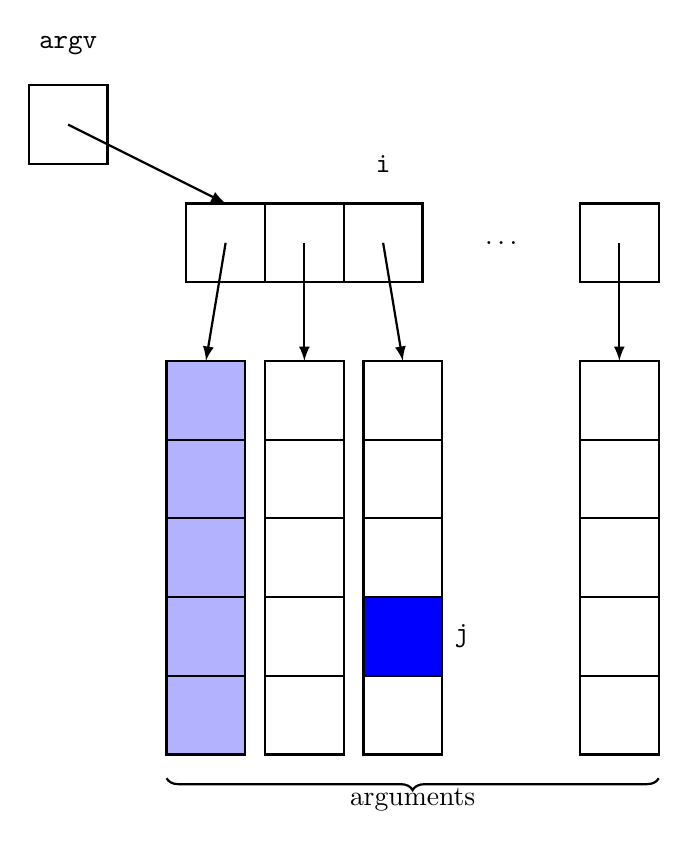
\begin{tikzpicture}
\tikzset{box/.style={draw,thick,minimum size=1cm,inner sep=0pt,outer sep=0pt}}
\tikzset{arrow/.style={->,>=latex,thick}}
\node [box] (argv) {};
\node at (2,-1.5) [box] (argv0) {};
\node at (3,-1.5) [box] (argv1) {};
\node at (4,-1.5) [box] (argv2) {};
\node at (5.5,-1.5) {$\ldots$};
\node at (7,-1.5) [box] (argv3) {};
\node at (1.75,-3.5) [box,fill=blue!30] (argv00) {};
\node at (3,-3.5)    [box] (argv10) {};
\node at (4.25,-3.5) [box] (argv20) {};
\node at (7,-3.5)    [box] (argv30) {};

\foreach \i/\j in {1/0,2/1,3/2,4/3}
{
  \node at (argv0\j.south) [anchor=north,box,fill=blue!30] (argv0\i) {};
}

\foreach \k in {1,...,3}
  \foreach \i/\j in {1/0,2/1,3/2,4/3}
  {
    \node at (argv\k\j.south) [anchor=north,box] (argv\k\i) {};
  }

\begin{scope}[on background layer]
\node at (argv23) [minimum size=1cm,inner sep=0pt,outer sep=0pt,fill=blue] {};
\end{scope}

\node at (0,1)    {\tt argv};
\node at (4,-0.5)    {\tt i};
\node at (5,-6.5) {\tt j};

\draw [arrow] (argv.center) -- (argv0.north);

\foreach \i in {0,...,3}
  \draw [arrow] (argv\i.center) -- (argv\i0.north);

\draw [thick,decorate,decoration={brace,mirror,amplitude=1ex}]
  ([yshift=-0.3cm]argv04.south west)
  -- node [below] {arguments} ([yshift=-0.3cm]argv34.south east);

\end{tikzpicture}
\end{document}

